% ---------------------------------------------------
%
% Trabajo de Fin de Grado. 
% Author: Laura Padrón Jorge. 
% Capítulo: La aplicacion BulletPoint. 
% Fichero: Cap4_TheApplication.tex
%
% ----------------------------------------------------
%

\chapter{La aplicación BulletPoint} \label{chap:laaplicacion} 

En este capítulo trataremos diversos temas relacionados con la aplicación, comenzaremos por definir posibles casos de uso en el ámbito universitario, tocaremos diversos temas relacionados incluyendo dificultades durante el desarrollo y acabaremos discutiendo posibles líneas futuras de desarrollo.

 
\section{Aplicaciones móviles en entornos universitarios}


Actualmente las posibilidades de las aplicaciones móviles para entornos universitarios se presentan amplias, cada universidad intenta tener su propia aplicación siguiendo un patrón similar. Realizando una investigación general de las aplicaciones disponibles en el mercado observamos que estas aplicaciones se centran en ofrecer servicios propios (servicio de correo, moodle, chat entre usuarios,etc), mantener al alumno informado y agilizarle los trámites principalmente. 

En un principio, estas aplicaciones se centraban en atraer alumnos, centrandose en la calidad de la universidad y mostrando las posibilidades que ofrecían, sin embargo con el paso de los años y el desarrollo creciente de las aplicaciones móviles, se muestra un cambio en esta estrategia. Ahora las aplicaciones tienen una doble función, no sólo buscan el acceso de nuevos estudiantes sino que también intentan mejorar la experiencia de los alumnos existentes y acercar a los nuevos a la experiencia de la universidad. 

Algunos ejemplos posibles los encontramos en el marketplace de google:

%No se si se pueden poner imagenes de aplicaciones universitarias en el marketplace.

Uno de los hechos que podemos observar es que las universidades están intentando obtener una solución rápida para desarrollar su app, una de las soluciones que se suelen adoptar es la creación de plantillas web optimizadas de su sitio web, lo que podemos considerar una opción rápida con un coste bajo.

En un futuro próximo con la aparición de los beacons, nos surge la pregunta ¿ Serán capaces estos dispositivos de transformar la educación ? De acuerdo con una encuesta realizado por %\textit{Software and Information Industry Association (SIAA)} \citeURL::SIAA%, casi todos los estudiantes hoy en día tienen acceso a un dispositivo móvil a través de %\textit{BYOD} \citeURL::BYOD%.El acercamiento de los estudiantes a los dispositivos móviles ha abierto la puerta a esta nueva tecnología.

\section {Posibles casos de uso de la tecnología beacon en entornos universitarios}

Como mencionaba antes, una de las posibilidades que se presentan para explotar esta tecnología se encuentra en las instituciones de enseñanza, las cuales podrían utilizar los beacons para facilitar a sus alumnos, profesores y demás personal involucrado  una serie de servicios de gran utilidad.

Sin embargo, para utilizar esta tecnología es necesario cumplir una serie de condiciones:

\begin{itemize}
\item Tener instalada la aplicación en su dispositivo móvil.
\item Tener activado el bluetooth.
\item La aplicación ha de estar despierta.
\item Las beacons han de estar desplegadas y configuradas correctamente en lugares clave donde el rango sea óptimo.
\end{itemize}

En el caso de dispositivos Apple no es necesario tener activado el bluetooth ya que el SO se encarga de captar las señales BLE, aparte tampoco es necesario que la app esté despierta ya que nuevamente el SO se encarga de despertar a la aplicación involucrada. Sin embargo Apple no ha desarrollado un IBeacon físico aún, aunque en un futuro, se espera que sus dispositivos móviles puedan funcionar como un beacon bidirecional.


Asimismo podemos afirmar que prácticamente hoy en día la mayoría de las universidades cuentan con una disposición amplia en los que se refiere a servicios y despliegue de medios. Como ejemplo podemos coger la Universidad de la Laguna, la cual cuenta con una red WiFi con un rango de cobertura casi completo de sus instalaciones y una amplia carta de servicios disponibles a sus alumnos por una serie de medios. Además cuenta con una serie de dispositivos beacons, que podrían ser instalados adecuadamente en lugares estratégicos. 

Partiendo de esta base, procederemos a explorar posibles casos de uso para los beacons en entornos universitarios tomando la ULL como referente:

\subsection{Guía a través del Campus de la ULL}

Este caso de uso cubre la funcionalidad destacada de un beacon, el posicionamiento y guia tanto en exteriores como en interiores. 

Como interesados podríamos destacar: 

\begin{itemize}
\item Personal invitado a jornadas o eventos en instalaciones de la ULL.
\item Alumnos de intercambio en programas internacionales.
\item Alumnos de nuevo acceso.
\item Personas con discapacidad.
\end{itemize}

\begin{figure}[h]
	\centering
	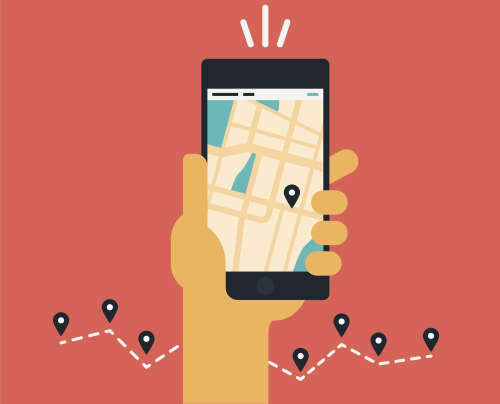
\includegraphics[width=\columnwidth]{locationMobileBeacon}
	\caption{Servicios de localización a través de la ULL}
	\label{fig:beaconLocation}
\end{figure}

El funcionamiento sería el siguiente: 

El usuario transita por las inmediaciones del campus universitario. En cuanto entra el el rango delimitado por el beacon, su movil vibra. El usuario mira su móvvil y ha recibido una notificación de la aplicación de la ULL. La notificación le informa que ha entrado en el rango del campus y si quiere entrar al sistema de navegación. Si el usuario acepta, la aplicación le muestra el camino mostrándole en todo momento su ubicación como un punto de color sobre el mapa de la ULL. Este mapa tiene marcados puntos de interés que contienen información de diferente tipo dependiendo del punto marcado, nombre, historia, página web, teléfono de contacto, trámites asociados a realizar,etc. El mapa se va actualizando dependiendo de la posición del usuario pudiendo volver a la vista más alejada en cualquier momento para una visualización más general.


\subsection{Descarga automática de material}

Este caso de uso resultaría muy útil para personal lectivo y para estudiantes, los cuales accederían de manera más sencilla al material dado. También sería aplicable para ponientes de charlas los cuales no tendrían que colgar sus apuntes en alguna plataforma externa o llevarlos consigo en  un almacenamiento externo para compartirlo al finalizar.

El funcionamiento sería el siguiente: 

El profesor o poniente lleva consigo un beacon y sus estudiantes u oyentes tienen instalados en sus dispositivos la aplicación. El profesor es capaz de introducir en su aplicación con el perfil de profesor (el poniente con su correspondiente perfil), indicaciones del material a utilizar en el evento. El profesor carga consigo el pequeño dispositivo e indica a sus alumnos que conecten el bluetooth y abran la aplicación, al entrar en el rango, la aplicación pedira permiso al alumno para descargarse el contenido indicado por el profesor. Si el alumno acepta, la aplicación pasaría a abrir  el contenido indicado por la página correspondiente.


\subsection{Acceso al parking y conteo de número de vehículos estacionados}


Este caso de uso proporcionaría información muy útil a los usuarios del parking de la universidad, informando del número coches estacionados en el parking y de las plazas restantes a ocupar en tiempo real.

El funcionamiento sería el siguiente: 

El personal de la Ull tendría la aplicación en su móvil, al acercarse a la barra del parking, el usuario activaría el bluetooth de su móvil. El beacon por su parte registraría un nuevo punto entrando en el rango de acción del parking. La aplicación comprobaría que el usuario está autorizado a entrar en el parking y procedería a abrir la puerta del parking dejando entrar al vehículo. Cuando el vehículo saliese del rango del beacon por el rango interior, la aplicación registraría entonces un nuevo acceso al parking y contabilizaría otro vehículo dentro de parking. Al salir del parking el proceso sería el mismo, por lo tanto la aplicación sería capaz de informar al usuario de las plazas ocupadas en tiempo real.


\subsection{Gestión de eventos e información, check in automático}

El funcionamiento sería el siguiente: 

Los alumnos transitan los interiores de la ULL de camino a sus clases. Los beacons están desplegados en las inmediaciones de lugares de interés, tipo aularium, paraninfo, clases que se utilicen a modo de salas de reuniones o seminarios. Al pasar por las inmediaciones de estos lugares de interés la aplicación alertaría al usuario de eventos que se celebrán en esos lugares, proporcionandole información de diversa índole, ponientes, tema de la charla, acceso, teléfono de contacto o otra información similar.  Al mismo tiempo la aplicación también cuenta con un tablón donde se muestran posibles eventos futuros. Estos eventos pueden ser muy variados y corresponder a diferentes tipos de actividades. Al mismo tiempo se podría confirmar la entrada al evento en el caso de haberla, mediante un código de acceso identificativo generado al realizar el pago del evento.

\subsection{Despacho del profesorado e información}

El funcionamiento podría abarcarse de dos maneras, por un lado, podría utilizarse para proveer a los alumnos de información acerca del grupo de despachos, aclarando que profesores tienen el despacho en la zona, horario de tutorías, correo electrónico de contacto, horario de corrección de exámenes, etc. De esta manera el alumno al acercarse a la zona sería capaz de saber información de todos los profesores, o si busca uno en particular la aplicación le da la opción de elegir su nombre de una lista y simplemente comprobar si tiene su despacho en esa zona. 

Por otro lado, este caso de uso podría abarcarse para proporcionar una información adicional, comprobando si el profesor está en la zona en ese momento y se encuentra disponible. El profesor tendrá un perfil de la aplicación con un código identificativo que le distingue de los demás profesores. Estos datos se guardarían en un servicio externo, y el beacon sería el encargado de registrar las entradas y salidas de los profesores. En cuanto al estado de disponibilidad, sería un dato que actualizaría el profesor desde su perfil de profesor en la aplicación. Los alumnos recibirían estos estados desde su lado de la aplicación y serían capaces de saber cuando el profesor se encuentra disponible mediante la aplicación. 

\subsection{Información y descuentos para usuarios de la APP}

Este caso de uso no solo dependería de la universidad sino de establecimientos comerciales interesados. La idea sería la siguiente: 

La universidad en colaboración con un establecimiento comercial le entrega un beacon. La aplicación contaría con un perfil para el dueño del establecimiento, donde sería capaz de introducir información que quiere que se muestre al usuario al pasar cerca de su establecimiento, mensajes de información, descuentos u ofertas especiales por ejemplo. El usuario al pasar por las inmediaciones del establecimeinto recibe en su aplicación una notificación del establecimiento con la información introducida por el dueño anteriormente. Al aceptar la notificación el usuario podría ser redirigido a la página web del establecimiento por ejemplo, para ver la oferta mejor o simplemente descartarla. En cualquier caso el establecimiento ha conseguido captar la atención de un posible cliente, y el usuario se benefiaría de ofertas y descuentos. 

\subsection{Control de asistencia}

Este caso de uso podría ir ligado al de Descarga automática de material, el funcionamiento sería el siguiente: 

El alumno conectaría el bluetooth de su móvil al iniciar la clase, en este momento la aplicación detectaría los dispositivos con los identificadores de alu de los alumnos y los dejaría registrados a la clase en el horario establecido. Los profesores serían capaces en todo momento desde su perfil de profesor de consultar asistencia. Si lo unimos con la descarga atomática de material proporcionaría comodidad tanto a alumnos como a profesores. Sin embargo un impedimento podría ser el rango del beacon o la necesidad de activar el bluetooth, ya que si  no tienes batería tendría que haber  un método secundario igualmente. 

\subsection{}

\section{4 Casos de uso elegidos}
%Arreglar una vez elija el caso de uso 


\section{Despliegue}


